\chapter{Control of driving speed (Extra)}%
\label{cha:contr-driv-speed}
As aforementioned, the planning dynamics is affected by the rate of fixed points
local shifts, as the system must be able to track the attractor as it
shifts, which effectively means that it is dependent on the path velocity, $v$.
Effectively, planning dynamics attractors and repellers are established as the
robot moves through the environment and sensory information 
changes or due to environmental changes (obstacles moving in the world). To keep
the system stable, i.e. in or near an attractor at all times, the rate of such
shifts must be limited to permit the track the attractor as it shifts. One way
of accomplishing this is by controlling the path velocity of the vehicle, as the
rate of fixed points shift is determined by the relative velocity of the robot
with respect to its environment~\cite{bicho2000dynamic}.

In this chapter, a more adequate dynamic system for path velocity is established
--- enhancing overall dynamics performance --- and analysed, assessing its
performance in several scenarios.

The maximal rate of shift of the fixed points as a function of the vehicle's
velocity is given by~\cite{bicho2000dynamic}:
\begin{equation}
  \label{eq:37}
  \dot\psi_{max} \approx \frac{\Delta \psi}{\Delta t} \approx \frac{v}{d}
\end{equation}

This approximate description can be turn around to compute the desired path
velocity as a function of distance with $\gls{psi-max-dot}$ as design parameter,
that can be tuned to obtain good tracking. The desired velocity is computed
separately for each of the two constraints ($j = \{tar, obs\}$)
~\cite{bicho2000dynamic}:
\begin{equation}
  \label{eq:38}
  \gls{V-j} = \gls{d-j} \dot \psi_{max}
\end{equation}

The desired velocities are imposed through a very simple dynamics~\cite{bicho1997dynamic}:
\begin{equation}
  \label{eq:39}
  \frac{dv}{dt} = 
- c_{obs}(v - V_{obs}) \exp \Big( - \frac{(v- V_{obs})^2}{2 \sigma_v ^2}  \Big)
- c_{tar}(v - V_{tar}) \exp \Big( - \frac{(v- V_{tar})^2}{2 \sigma_v ^2}  \Big)
\end{equation}

The strengths, $\gls{c-obs}$ and $\gls{c-tar}$, are tuned such that in the presence of
strong obstacle contributions the obstacle term dominates while in the absence
of such contributions the reverse holds. A systematic way to construct a
function that indicates if obstacles contributions are present, is to integrate
force-lets, from which a potential function of the obstacle avoidance dynamics
results~\cite{bicho2000dynamic}:
\begin{equation}
  \label{eq:40}
  U(\phi) = \sum_{i = 1}^N{ \Bigg( \lambda_i \sigma_i^2  \exp \Big( - \frac{ (\phi -\psi_i)^2 }{2 \sigma_i ^2} \Big) - \lambda_i \frac{\sigma_i ^2}{\sqrt{e}}  \Bigg)  }
\end{equation}

Positive values of this potential function indicate that the heading direction
is in a repulsion zone of sufficient strenght, $\lambda_i$, so $c_{obs} > 0$ and
$c_{tar} = 0$ is required. Conversely, negative values of the potential indicate
that the heading direction is outside the repulsion range or repulsion is weak,
so now $c_{obs} = 0$ and $c_{tar} > 0$ is required~\cite{bicho2000dynamic}. 
Effectively:
\begin{equation}
  \label{eq:41}
  U(\phi) = \left\{
\begin{array}{ll}
      < 0 , & c_{obs} = 0 \wedge c_{tar} > 0 \quad \rightarrow \quad \mathrm{attractor} \\
      > 0 , & c_{obs} > 0 \wedge c_{tar} = 0 \quad \rightarrow \quad \mathrm{repeller} \\
\end{array} 
\right. 
\end{equation}

The transformation of potential levels to the strengths of the two contributions
to the velocity control makes use of a sigmoidal threshold
function~\cite{bicho2000dynamic}:
\begin{equation}
  \label{eq:42}
  \alpha(\phi) = \frac{\arctan(c U(\phi))}{\pi}
\end{equation}
ranging from $-1/2$ to $1/2$ (see Fig.~\ref{fig:lyapunov}, withdrawn from~\cite{bicho2000dynamic}). 
%
\begin{figure}[!hbt]
\centering
    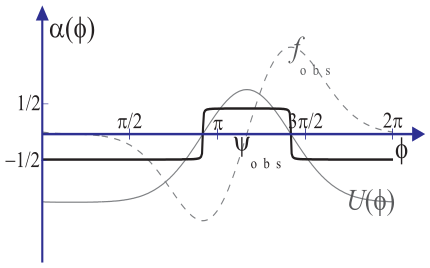
\includegraphics[width=0.5\textwidth]{./img/lyapunov.png}
  \caption[Control of driving speed: threshold potential, potential and
  repulsive force-let (withdrawn from~\cite{bicho2000dynamic})]{The dashed line
    is a repulsive force-let, $f_{obs}$. Its integral provided a potential
    (solid thin line), $\gls{U}$, which is maximal near the heading direction to be
    avoided, i.e., resultant repeller. The thresholded potential (solid bold
    line), $\gls{alpha}$, serves as an indicator of those intervals of the heading
    direction from which obstacle forces repel (withdrawn from~\cite{bicho2000dynamic})}%
\label{fig:lyapunov}
\end{figure}

Finally, the following functions for
the strenghts of the two velocity contributions can be written:
\begin{equation}
  \label{eq:41}
\begin{array}{ll}
      c_{obs} = c_{v,obs} (1/2 + \alpha(\phi) ) \\
      c_{tar} = c_{v,tar} (1/2 - \alpha(\phi) ) \\
\end{array} 
\end{equation}

At sufficiently sharp sigmoids ($\gls{C}$ sufficiently large) this leads to the
required transition behavior. The parameters, $\gls{c-v-tar}$ and $\gls{c-v-obs}$,
determine the relaxation rate of the velocity dynamics in the two cases when
either the obstacle or the target constraints dominate~\cite{bicho2000dynamic}. 

The following hierarchy of relaxation rates ensures that the system relaxes to
the attractors and that obstacle avoidance has precedence over the target
contribution~\cite{bicho2000dynamic}:
\begin{equation}
  \label{eq:43}
  \lambda_{tar} \ll c_{v,tar},
  \quad
  \lambda_{obs} \ll c_{v,obs},
  \quad
  \lambda_{tar} \ll \lambda_{obs}
\end{equation}

\section{Implementation}%
\label{sec:implementation-lyapunov}
Following the guidelines presented in the previous section, the overall dynamics
with control of the driving speed was implemented. The first order differential
equation for path velocity --- Eq.~(\ref{eq:39}) --- was converted into an
algebraic recursive equation, using forward Euler's method. 

The potential function, $U(\phi)$, and thresholded potential function, $\alpha(\phi)$,
were computed as an intermediate step.
It should be noted that if no contributions from obstacles are present, then
$\alpha(\phi) = 0$, yielding both obstacles and target contributions to the path
velocity, i.e., that are two attractors for the dynamics. However, in the
beginning the initial velocity of the robot is very low, resulting in a
neglectable aceleration, thus causing the robot to move at this constant
velocity until it detects the presence of obstacles. To prevent this, if
$\alpha(\phi) = 0$, the robot moves at a reasonable constant speed.

Additionally, to assist the tuning of the parameters and the comprehension of
the overall dynamics with control of the driving speed, the potential,
$U(\phi)$, and thresholded potential ($\alpha(\phi)$) functions are plotted
alongside with the obstacle avoidance and target acquisition dynamics.

As a result, the following generic Matlab code was implemented (Listing~\ref{lst:program-dyn-obs-tar-lyapunov}):
% program_dyn_tar.m (generic)
\lstinputlisting[language=matlab, caption={Generic implementation of the overall
  dynamics with control of driving speed (not tuned)},label=lst:program-dyn-obs-tar-lyapunov,
style=custom-matlab]{./listing/program_dyn_obs_tar_lyapunov.m}%
%
\section{Simulations}%
\label{sec:sim-lyapunov}
Several simulations were performed to tune the multiple parameters and to assess
the performance of the overall planning dynamics with control of driving speed.

\subsection{Tuning}%
\label{sec:tuning-lyapunov}
The parameters were then tuned, starting from the hierarchy of relaxation rates that
ensures that the system relaxes to the attractors and that obstacle avoidance
has precedence over the target, imposed as:
%
\begin{lstlisting}[language=matlab, caption={Relaxation rates tuning},label=lst:program-dyn-lyapunov-relax-tuning,
style=custom-matlab]%

   %% obstacle
   tau_obs_min = 3.5 * dt; % flexible
   beta1 = 1/tau_obs_min; %  = lambda_obs_max = 1/tau_obs_min
   %% target
   tau_tar = 20*tau_obs_min; % relaxation time for attractor
   lambda_tar = 1/tau_tar; % attraction magnitude
   %% velocity
   c_v_obs = 10 * beta1; % obstacle contribution to velocity
   c_v_tar = 100 * lambda_tar; % target contribution to velocity

\end{lstlisting}

Next, the parameters directly related to the path velocity dynamics were tuned,
as follows:
%
\begin{lstlisting}[language=matlab, caption={Path velocity parameters tuning},label=lst:program-dyn-lyapunov-veloc-tuning,
style=custom-matlab]%

   % Lyapunov
   Rtar = 20; % target radius
   d_min = Rrobot + Rtar + 5; % minimum distance to target
   C = 100; % potential constant
   d_obs = d_min; % minimum distance to obstacle
   d_tar = d_min; % minimum distance to target
   psi_max = pi/12; % maximum rate of fixed points shift
   sigma_v = pi/6; % angular range for velocity
   Vobs = d_obs * psi_max; % maximum velocity for obstacle avoidance behavior
   Vtar = d_tar * psi_max; % maximum velocity for target acquisition behavior

\end{lstlisting}
The potential constant, $C$, was defined high enough to obtain a sharp sigmoid,
required for the transition behavior. The distance to obstacle and target were
considered as the minimum one, corresponding to the robot's size. The maximum
rate of fixed points shift,$\dot \psi_{max}$, was set to a relatively small
value, so the system can closely follow the attractors. The angular range for
velocity, $\sigma_v$, defines the range where the obstacles presence must be
accounted for path velocity dynamics,and this was set to two sensor sectors.

\subsection{S scenario}%
\label{sec:s-scenario-lyapunov}
Then, the robot's planning dynamics was simulated using the
\texttt{MobileRobotDyn\_Tar\_Obs\_S.ttt} scenario (see Fig.~\ref{fig:lyapunov-s}
and Video \href{run:./videos/lyapunov-s.mp4}{./videos/lyapunov-s.mp4}). 
%
\begin{figure}[htb!]
  \centering
%
  \begin{subfigure}{.7\textwidth}
    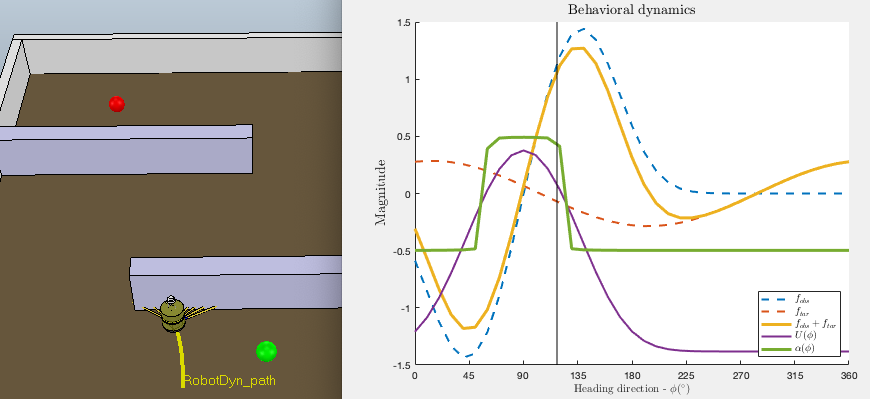
\includegraphics[width=\textwidth]{img/lyapunov-s-1.PNG}%
  \caption{}%
  \label{fig:lyapunov-s-1}
  \end{subfigure}
%
  \begin{subfigure}{.7\textwidth}
    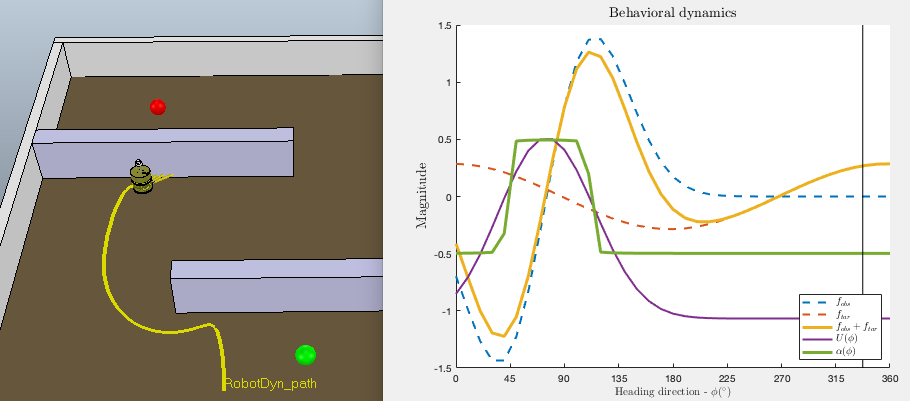
\includegraphics[width=\textwidth]{img/lyapunov-s-2.PNG}%
  \caption{}%
  \label{fig:lyapunov-s-2}
  \end{subfigure} 
  % 
  \begin{subfigure}{.7\textwidth}
    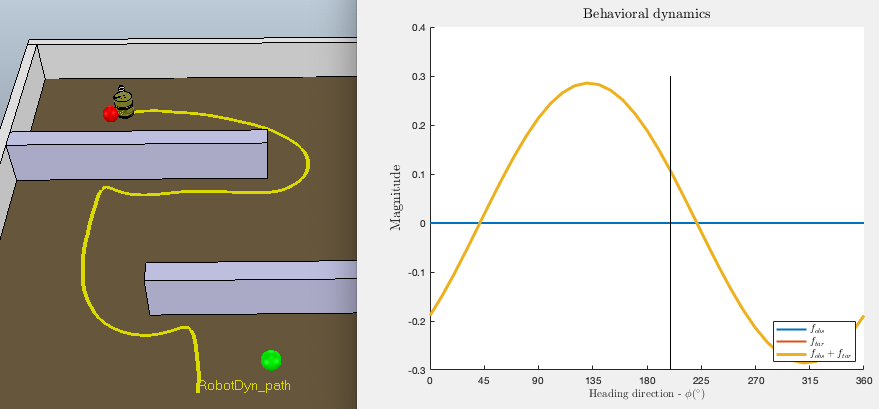
\includegraphics[width=\textwidth]{img/lyapunov-s-3.PNG}%
  \caption{}%
  \label{fig:lyapunov-s-3}
  \end{subfigure}
%
  \caption{Planning dynamics with control of driving speed: Scenario S}%
  \label{fig:lyapunov-s}
\end{figure}
%
The robot moves initially with a constant, predefined, speed, with a slight tilt
due to the orientation of the target, $\psi_{tar}$. When the robot approaches
the wall, the obstacles are
detected in a significant way (Fig.~\ref{fig:lyapunov-s-1}), with the overall
dynamics establishing a repeller on the 90 degrees heading
direction. Consequently, the obstacles potential is positive in the vicinity of
the repeller, i.e. $U(\phi) > 0$, and, thus, the thresholded potential is also
positive, i.e. $\alpha(\phi) > 0$, with the defined angular range
$\sigma_v$. Hence, the robot starts to turn left --- $\phi > 90 ^{\circ}$ ---
with the path velocity defined by Eq.~(\ref{eq:39}), affected by the sigmoidal
function and the associated parameters.

Fig.~\ref{fig:lyapunov-s-2} shows a similar situation, but now the robot turns
right --- $\phi \approx -45 ^{\circ}$. Lastly, Fig.~\ref{fig:lyapunov-s-3}
illustrates the final state of the simulation when the robot reaches the target,
and only its contribution is present. There is slight mismatch between the
heading direction and the closest attractor due to the imposed path velocity
dynamics. Comparing this simulation to the nonlinear dynamics for heading
direction with linear path velocity dynamics
(Fig.~\ref{fig:obs-tar-nonlinear-scenario2}), it can be observed a more `clean'
and shortest path, although with greater cornering radius, due to the increased
average speed.

\subsection{Tar-Obs Scenario}%
\label{sec:tar-obs-scenario-lyapunov}
Then, the robot's planning dynamics was simulated using the
\texttt{MobileRobotDyn\_Tar\_Obs.ttt} scenario with a 50 cm gap between
obstacles (see Fig.~\ref{fig:lyapunov-tar-obs} and 
Video \href{run:./videos/lyapunov-tar-obs.mp4}{./videos/lyapunov-tar-obs.mp4}). 
%
\begin{figure}[htb!]
  \centering
%
  \begin{subfigure}{.49\textwidth}
    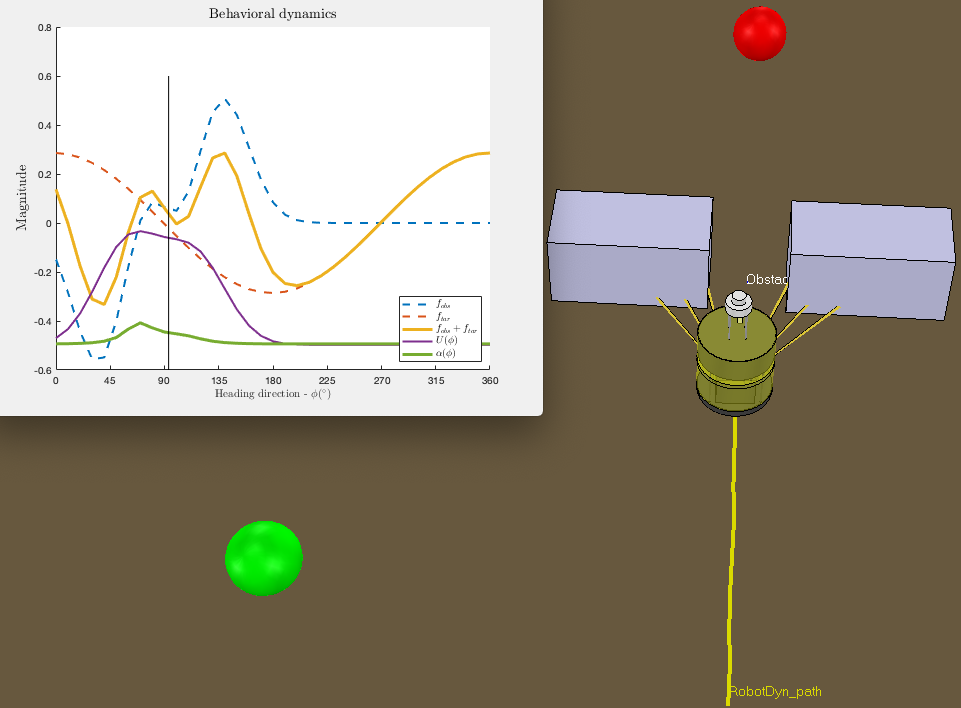
\includegraphics[width=\textwidth]{img/lyapunov-tar-obs-1.PNG}%
  \caption{}%
  \label{fig:lyapunov-tar-obs-1}
  \end{subfigure}
%
  \begin{subfigure}{.49\textwidth}
    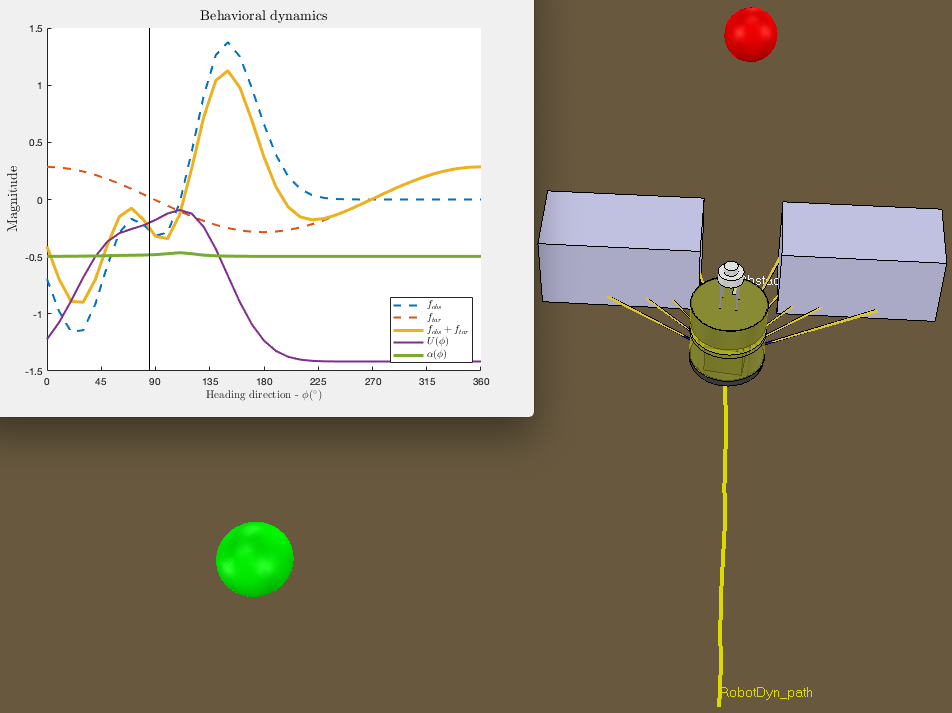
\includegraphics[width=\textwidth]{img/lyapunov-tar-obs-2.PNG}%
  \caption{}%
  \label{fig:lyapunov-tar-obs-2}
  \end{subfigure} 
  % 
  \begin{subfigure}{.49\textwidth}
    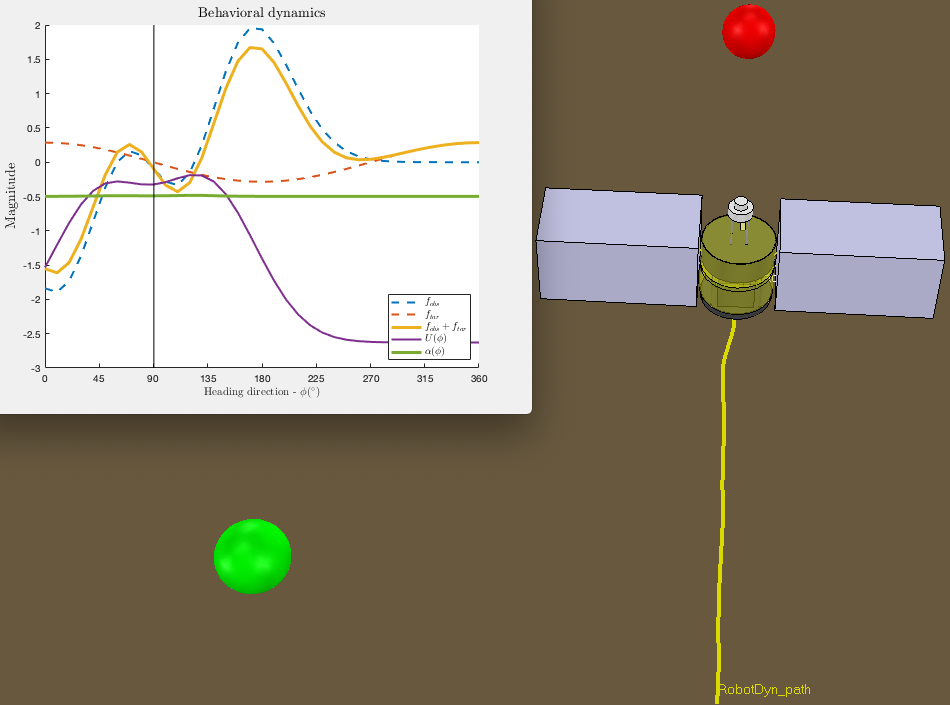
\includegraphics[width=\textwidth]{img/lyapunov-tar-obs-3.PNG}%
  \caption{}%
  \label{fig:lyapunov-tar-obs-3}
  \end{subfigure}
  % 
  \begin{subfigure}{.49\textwidth}
    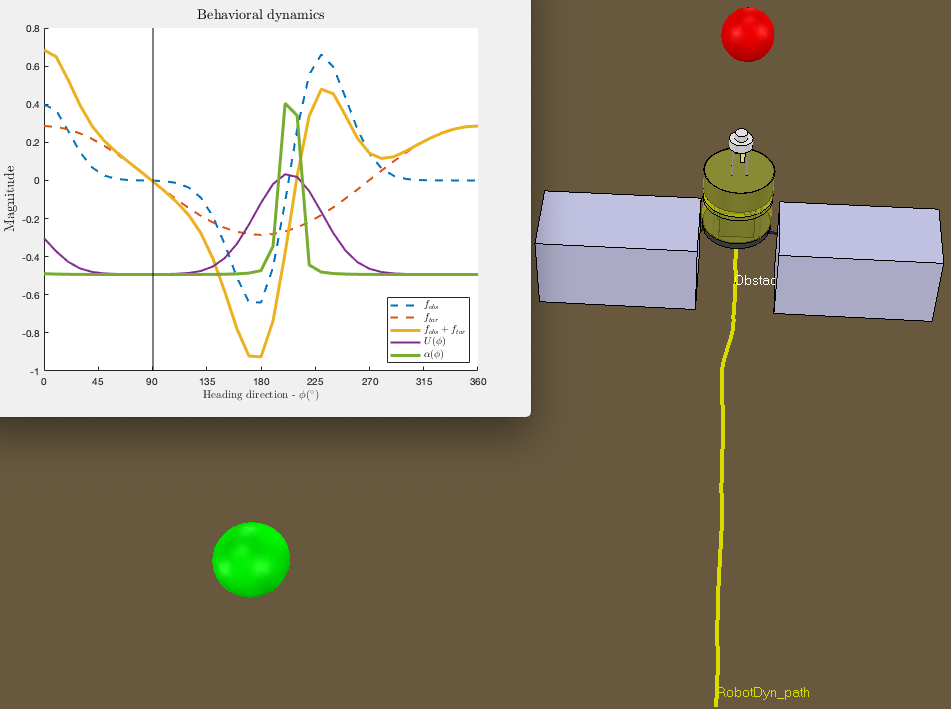
\includegraphics[width=\textwidth]{img/lyapunov-tar-obs-4.PNG}%
  \caption{}%
  \label{fig:lyapunov-tar-obs-4}
  \end{subfigure}
  % 
  \begin{subfigure}{.49\textwidth}
    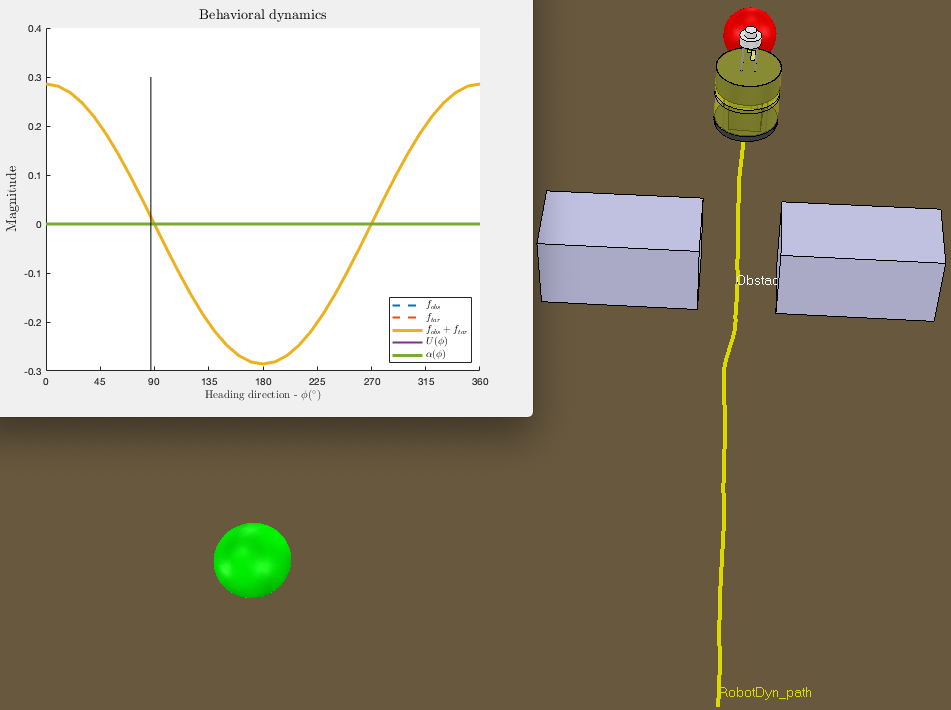
\includegraphics[width=\textwidth]{img/lyapunov-tar-obs-5.PNG}%
  \caption{}%
  \label{fig:lyapunov-tar-obs-5}
  \end{subfigure}
%
  \caption{Planning dynamics with control of driving speed: Scenario Tar-Obs}%
  \label{fig:lyapunov-tar-obs}
\end{figure}

The robot moves forward, towards the target, until it starts to detect the
obstacles (Fig.~\ref{fig:lyapunov-tar-obs-1}). Although the potential function
is not null, it is negative as expected, as the target acquisition behavior is
prevalent --- an attractor is established in the heading direction. Thus, only
the target contributes to the path velocity
dynamics. Fig.~\ref{fig:lyapunov-tar-obs-2} and
Fig.~\ref{fig:lyapunov-tar-obs-3} illustrate a similar behavior, although with
slight variations in the potential function, as the robot moves in between the
obstacles. Fig.~\ref{fig:lyapunov-tar-obs-4} showcases the only brief moment
when the thresholded potential is positive, i.e. $\alpha(\phi) > 0$, as the
robot escapes the obstacles wall and the obstacle avoidance prevails over the
target acquisition behavior for the path velocity dynamics. Lastly,
Fig.~\ref{fig:lyapunov-tar-obs-5} shows the moment the robot reaches the target
with an attractor in the heading direction as expected. This simulation
showcases a critical scenario, where the robot must pass between the obstacles
at a minimum distance, yet, at a adequate velocity.
%
%
\section{Discussion}%
\label{sec:discussion-lyapunov}
The control of driving speed is critical for maintaing the stability of the
planning dynamics of the robot, as it limits the rate of fixed points shifts,
enabling the system to track the attractor as it shifts.

The shifting of fixed points for the planning dynamics can stem from robot
movement through the environment and associated sensory information 
changes or due to environmental changes (obstacles moving in the world), causing
attractors and repellers to change. To keep
the system stable, i.e. in or near an attractor at all times, the rate of such
shifts must be limited to permit the track the attractor as it shifts. One way
of accomplishing this is by controlling the path velocity of the vehicle, as the
rate of fixed points shift is determined by the relative velocity of the robot
with respect to its environment~\cite{bicho2000dynamic}.

In this chapter, a more adequate dynamic system for path velocity was
established, as the sum of obstacles and target contributions, where one of the
components dominates at all times. A systematic way to construct a
function that indicates if obstacles contributions are present, is to integrate
force-lets, from which a potential function of the obstacle avoidance dynamics
results. If the potential is positive a repeller is established for the planning
dynamics, and conversely, if negative an attractor arises. A convenient way 
to transform the potential levels to the strengths of the two contributions
to the velocity control is through the use of a sigmoidal threshold function,
defining the angular range the obstacles contribution is noticeable.

Then, the parameters were tuned considering the hierarchy of relaxation rates
--- which ensures that the system relaxes to the attractors and that obstacle
avoidance has precedence over the target --- and some rules of thumb for the
remaining path velocity parameters.

Finally, two scenarios were simulated --- S and Tar-Obs --- to assess the
performance of the overall dynamics. It was shown that, although the average
velocity was increased, the planning dynamics remains robust, suggesting a performance improvement in the overall dynamics.
%%% Local Variables:
%%% mode: latex
%%% TeX-master: "../../dissertation"
%%% End:
